%!TEX root = ../main_wo_rep.tex
%
% 光の性質
%


\section{光の性質}

\subsection{光の波動性}

\begin{itemize}

\item 光は光速度$c$の速さで伝わる波です。\\
(真空中の光速度:$c=2.99792458\times 10^8$ [m/s])\\
性質1. 横波です。\\
性質2. 他の波と同様に、屈折、反射、回折、干渉が起きます。\\
性質3. 他の波と異なり、真空中(媒質が無い所)でも伝わります。

\item 人間の目は、光のうち波長が約400 [nm]〜約800 [nm]のものを「色」で区別するこ
とができ、波長の長い光は赤色、波長の短い光は紫として認識します。\\
$\Rightarrow${\bf [実験 2-1, 2-2]}

\begin{center}
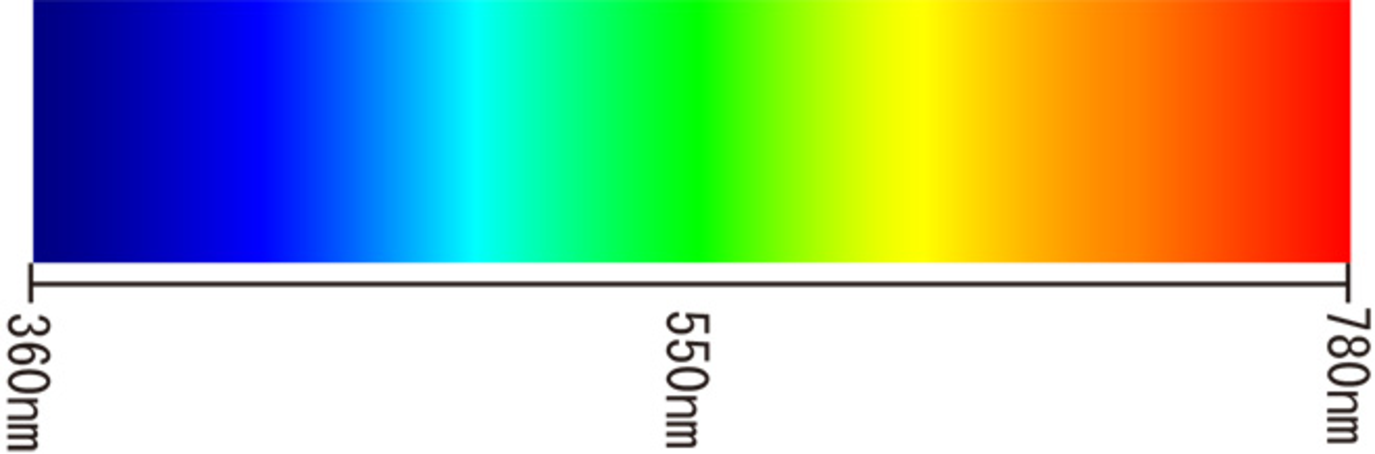
\includegraphics[scale=0.6, bb=0 0 660 218]{02_Refraction/spectrum.pdf}
\end{center}

\end{itemize}



\bigskip

\begin{itembox}[l]{\bf コラム:光速度より遅い光}
光速度$c=2.99792458\times 10^8$ [m/s]は真空中を進む光の速度です。物質中を進む光の速 
度は光速度$c$より遅くなります。光は速過ぎて(1秒間に地球を7周半もする速さ!)扱いづら 
いので、光をできるだけゆっくり進むようにさせたいという研究が行われています。今の 
ところ、実験段階で達成された一番遅い光の速度は、シリコンを主とした物質内を通る 
光の速度で、真空中の光速度$c$の300分の1ほどしかありません。
\end{itembox}

\newpage

\subsection{光の反射と屈折}

\subsubsection{屈折率}

\begin{wrapfigure}[8]{r}{5cm}
\vspace*{-0.8cm}
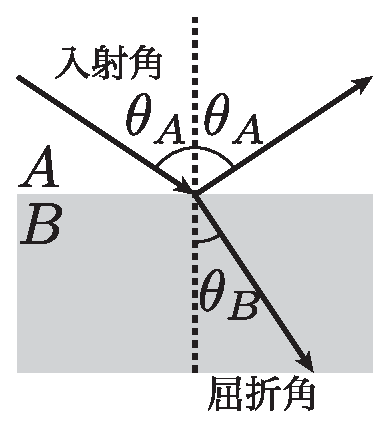
\includegraphics[scale=0.8]{02_Refraction/refraction.eps}
\end{wrapfigure}


密度の違う2つの媒質A、Bが隣り合っているとします。光が媒質Aから媒質Bの方
向に、斜めに入射する場合を考えましょう。

光の一部はAとBの境界面で反射し、また一部は屈折・透過して媒質Bの中を進みます。この時の、
媒質BのAに対する屈折率は次のようになります。
\[
n_{\rm AB} = \frac{n_{\rm B}}{n_{\rm A}} = \frac{\sin \theta_A}{\sin \theta_B}
\qquad
\left(
n_{\rm BA} = \frac{n_{\rm A}}{n_{\rm B}}=\frac{1}{n_{\rm AB}}
\right)
\]
\begin{eqnarray}
n_{\rm A} & \cdots & \text{媒質Aの絶対屈折率(真空に対する屈折率)}\nonumber\\
n_{\rm B} & \cdots & \text{媒質Bの絶対屈折率}\nonumber
\end{eqnarray}
ただし、空気の絶対屈折率は、$n = 1.0003$なので、$n=1$として計算してかまいません。
([媒質の空気に対する屈折率]=[媒質の絶対屈折率] と考えて良い。)

屈折率は光の波長によって異なり、波長が短い光ほど屈折率が大きくなります。すなわち、
赤い光よりも紫の光の方が大きく屈折します。$\Rightarrow${\bf [実験 2-1, 2-2]}

\subsubsection{全反射}

光を、屈折率の大きい媒質Aから屈折率の小さい媒質Bに向けて入射させることを
考えてみましょう。この場合は、入射角より屈折角の方が大きくなります。このとき、入射角が小
さいうちは、入射光の多くは屈折していきますが、入射角を大きくしていくと、ある角度
で屈折角が$90^\circ$になり、これより大きい入射角では光線は媒質Aに進入できず、全
て境界面で反射するようになります。これを{\bf 全反射}といいます。$\Rightarrow${\bf [実験 2-3, 2-4]}

全反射(屈折角が$90^\circ$より大きくなる)が起こるようになる入射角を{\bf 臨界角}といいます。臨界
角は次の式で求められます。$\Rightarrow${\bf[実験 2-4]} 
\begin{eqnarray}
&&n_{\rm A}\sin\theta_A = n_{\rm B} \sin 90^\circ\nonumber\\
&& \Rightarrow \sin\theta_A = \frac{n_{\rm B}}{n_{\rm A}}\nonumber
\end{eqnarray}

\subsubsection{糖度計}

糖度計は測定対象となる液体に含まれる糖の含有量によって光の屈折率が異なる事を利用して
果物等の糖度を測定する装置です。正確には屈折糖度計と呼びます。
糖度とは液体に含まれるショ糖の質量パーセント濃度のことで、Brix\%(ブリックス)
という単位で表します。レモンのように糖度が高くても酸味が強ければ、それほど
甘く感じないので、糖度が感覚的な甘さを表すとは限りません。


\begin{figure}[h]
\begin{center}
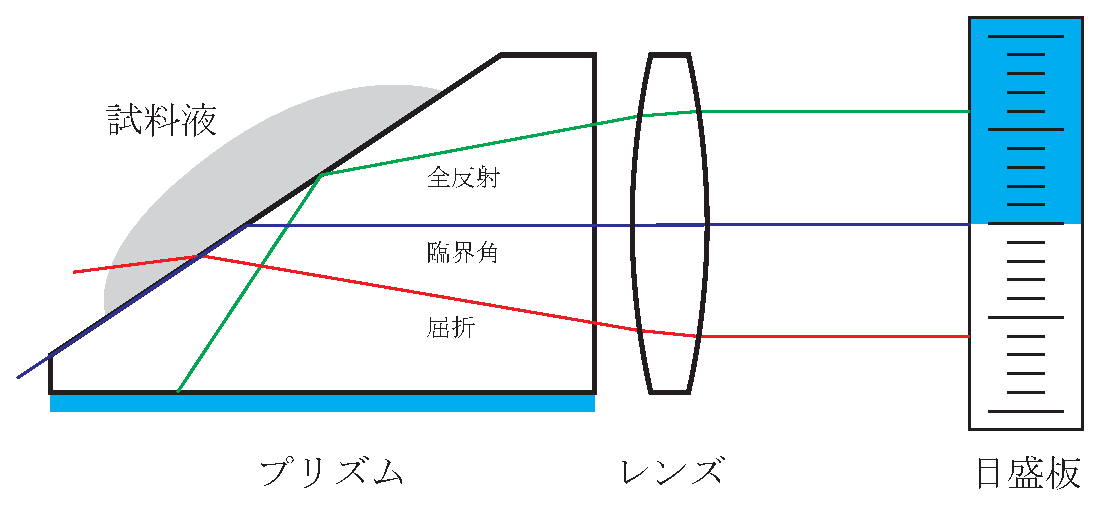
\includegraphics[scale=0.75]{02_Refraction/brix.eps}
\end{center}
\caption{糖度計の仕組み}
\end{figure}

\subsubsection{偏光}

光は進行方向に対して垂直に振動する横波であり、その振動方向が偏ったものを{\bf 偏光}と呼びます。
太陽光などの自然の光は振動方向がまちまちで偏光していませんが、偏光子
と呼ばれる特別な材質のものに光を透過させると、特定の偏光の成分を取り出すことができます。

偏光子を通した光は振動方向が特定の方向になっており、その光をもう一度偏光子を通した場合、
相対的な偏光の方向によって明るさが変化します。
このような偏光の性質を用いて、光の透過率を電気的にコントロールすることができ、
偏光は液晶ディスプレイなどに応用されています。

偏光子には方解石など自然に産出される物質もありますが、現在では偏光フィルムのように
高分子を用いて、安く大量に作ることができるようになり、工業的な利用が進んでいます。




\bigskip
\bigskip

\begin{itembox}[l]{\bf コラム1:光海底ケーブル}
光海底ケーブルは、複数本の光ファイバーケーブルをアルミニウムや鉄芯で耐圧性を高
めたものにポリエチレンで覆いをしたものです。世界中で約80万[km]ものケーブ
ルが海底に巡らせてあります。2005年の時点で、太平洋を横断している光海底ケーブルのシ
ステムは6つで、その全容量は10[Tbps]にも達しますが、そのうち実際に使用されてい
るのは1[Tbps]にとどまっているのが現状です。島国である日本の国際通信の多くは
このような海底ケーブルを利用して行われています。\\
 ※1[Tbps] =1,000,000,000,000 [bps] = 1,000,000,000,000 [ビット/秒] 
\end{itembox}

\bigskip

\begin{itembox}[l]{\bf コラム2:いろいろな糖度計}
屈折糖度計の他にも糖度を測る方法がいろいろあります。旋光糖度計は、ショ糖に
特定の偏光を持った光を通すとその光の偏光面を$66.5^\circ$回転させるという
旋光性を利用して糖度を測るものです。近赤外光糖度計は、ショ糖が近赤外光を吸収する
性質を利用して近赤外光の吸収度合いを測定して糖度を求めるものです。
果物などの作物の糖度を測る場合、屈折糖度計も旋光糖度計もサンプルを傷つけ果汁
を絞り取る必要がありますが、近赤外糖度計はサンプルを傷つけることなく糖度を測定できるので、
分光技術の進歩にともなう装置の小型化と相まって、利用が広がっています。
\end{itembox}

\newpage

\jikken

\begin{itemsquarebox}[c]{\bf 実験用具}
分光用プリズム、白熱灯光源装置、半導体レーザー光源装置、アクリルブロック、
光ファイバー結束線、ファイバースコープ、
光学水槽、糖度計、偏光フィルム、セロハンテープ、方解石
\end{itemsquarebox}

\bigskip

\subjikken{白色光}

太陽光や白熱灯の光は多くの異なる波長の光を含んでいます。白熱灯光源装置の光
をプリズムに入射させると、波長の異なる波は、屈折率の違いによって分散します。
この分散した波長スペクトルを白壁に投影して観察してみましょう。
正三角形のプリズムと直角のプリズムでスペクトルの現れ方(色の順番)に違いが出るでしょうか?
\begin{center}
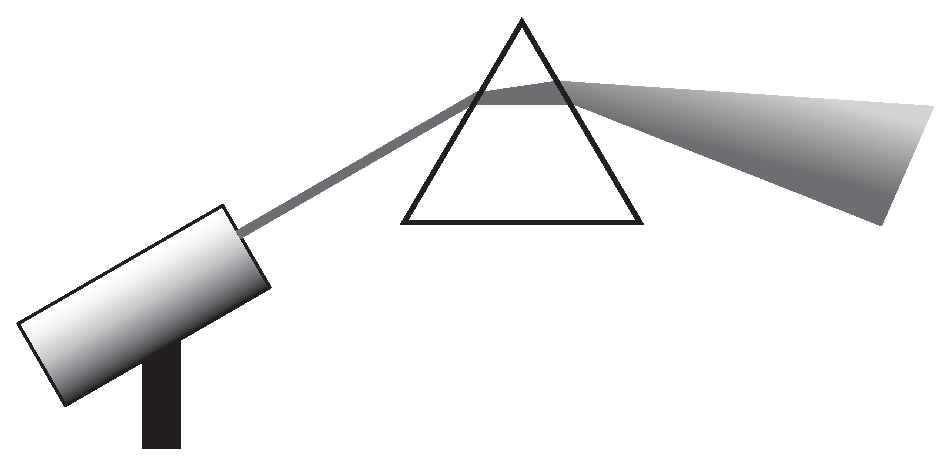
\includegraphics[scale=0.4]{02_Refraction/prism.eps}
\end{center}


\subjikken{単色光}

レーザー光は、ある特定の波長の光のみを、ビームとして出しています。レーザー
光源装置の光を、{\bf [実験 \thesection-1]}と同様に、プリズムを通して観察し、レーザー光が
単一波長の光(単色光)であることを確かめましょう。

\bigskip


\subjikken{光の屈折と反射}

様々な形をしたアクリルブロックにレーザー光を入射させて反射と屈折の法則を確認しましょう。

\bigskip

\subjikken{光ファイバー}

細長い、あるいはS字型のアクリル棒を使って、レーザー光が内部で全反射を起こすこと(条件)を確かめましょう。この光ファイバーの原理を応用した光ファイバー結束線やファイバースコープを使って、光ファイバーの働きを確認しましょう。

\bigskip

\subjikken{臨界角}

光学水槽を用いて、水中から空気中に向けてレーザー光を入射させ、全反射が起こ
ることを確かめましょう。また、このときの臨界角を読み取り、水の屈折率を求めま
しょう。

\bigskip


\newpage

\subjikken{糖度計}

糖度計を用いてコーラやジュースの糖度を計ってみましょう。液体のサンプルをスポイトを使って
糖度計のプリズム面に少量たらし、ふたをしてサンプルがプリズム面に均一に行き渡るようにします。
糖度計を水平に保ちながら接眼部からのぞき、青と白の境界線の目盛の数値から糖度(Brix)
を読み取りましょう。

\bigskip


\subjikken{偏光フィルム}

偏光フィルムを2枚用意して重ね合わせ光が透過する様子を観察しましょう。
重ね合う角度を変化させると透過する光の明るさはどうなるでしょうか。
携帯電話の液晶画面、方解石、様々なものを反射した光などを偏光フィルムを通して見てみましょう。
また、2枚の偏光フィルムの間にセロファン(セロファンテープ)を
重ねて挟んで色や明るさの変化を見てみましょう。

\bigskip



\hspace*{-\parindent}
{\bf 注意}:\underline{レーザー光源を直接目に入れてはいけません。}(ビームの出口をのぞき込まな 
いこと!) 間違って他人の顔の方向にレーザー光を向けてしまわないように、
ビームの出る方向に人がいないことを確認してから電源を入れるようにしましょう。


